
\documentclass[11pt]{article}
\usepackage[letterpaper,margin=0.92in]{geometry}
\usepackage[T1]{fontenc}
\usepackage[utf8]{inputenc}
\usepackage{lmodern}
\usepackage{microtype}
\usepackage{parskip}
\usepackage{enumitem}
\usepackage{booktabs}
\usepackage{tabularx}
\usepackage{array}
\usepackage{hyperref}
\usepackage[round]{natbib}
\usepackage{xcolor}
\usepackage{fancyhdr}
\usepackage{amsmath}
\usepackage{amssymb}
\usepackage{tikz}
\usetikzlibrary{arrows.meta,positioning,fit}
\setlength{\parindent}{0pt}
\setlength{\headheight}{14pt}
\hypersetup{colorlinks=true,linkcolor=black,citecolor=black,urlcolor=black}
\sloppy
\pagestyle{fancy}
\fancyhf{}
\lhead{\small When Words Stop Being the Cause}
\rhead{\small Working Paper}
\cfoot{\thepage}

\newcommand{\paperstatus}{Rival-Mechanisms Working Paper}
\newcommand{\markbox}{\raisebox{-0.35em}{
\includegraphics[width=0.32in]{MARK.svg}}}

\begin{document}

\begin{center}
{\LARGE\bfseries When Words Stop Being the Cause}\\[0.35em]
{\large The Causal Attribution Problem in Prompted Generative Systems}\\[0.7em]
{\normalsize Watson Hartsoe}\\
{\small \paperstatus\ --- 17 August 2026}
\end{center}

\vspace{0.5em}

\begin{abstract}
Prompt practice is usually narrated as if a visible instruction causes a generated artifact: change the words, observe the output, and infer what the prompt did. That inference is increasingly difficult to justify. Deployed systems may rewrite a user's request before generation; prompt compilers can synthesize the text actually executed; continuous ``soft prompts'' can control a model without readable words; human nonwords and single Unicode substitutions can nonetheless have strong model-relative effects; concepts can appear in early diffusion attention and disappear before the final image; initial random state can exhibit reproducible content preferences; and adding explicit requirements can reduce rather than increase instruction following. These findings do not support one replacement ontology of ``the prompt.'' They expose a causal-attribution problem. The same surface relation---a prompt followed by an apparently responsive output---is compatible with several rival mechanisms operating at different stages. This paper develops that underdetermination as a research problem. It distinguishes surface-semantic, transformation, distributed-dynamical, and selection accounts of prompt effects, shows why ordinary prompt-output comparison often cannot discriminate among them, and proposes an intervention ladder for locating control across user text, rewriting, representation, generative dynamics, stochastic state, and evaluation. The central question is therefore not whether prompts are programs. It is narrower and harder: under what conditions are the words visible to the user actually the cause of what the system does?
\end{abstract}

\noindent\textbf{Keywords:} prompting; generative systems; causal attribution; text-to-image; prompt programming; model interpretation; stochastic generation; prompt optimization

\vspace{0.6em}
\hrule
\vspace{0.35em}
\begin{flushright}
\scriptsize AI-augmented working paper. Research and assembly record accompanies the publication.
\end{flushright}
\vspace{0.2em}

\section{A sentence and a causal claim}

A prompt interface stages a persuasive little experiment. A person writes a sentence. A system returns an artifact. The screen places the two next to each other. Change the sentence and the artifact changes. It is natural to say that the words caused the result.

Much of prompt practice depends on some version of this attribution. Prompt engineering assumes that revisions to wording can improve behavior. Prompt programming treats some natural-language instructions as components of software systems \citep{Liang2025PromptsPrograms}. Languages such as LMQL explicitly combine textual prompting with scripting, control flow, and output constraints \citep{BeurerKellner2023LMQL}. Experimental tools such as ChainForge make prompts into variables by comparing responses across prompt variants and models \citep{Arawjo2023ChainForge}. All of these practices require prompt differences to be meaningful interventions.

But ``the prompt caused the output'' is not a description of an observable sequence. It is a causal claim. The observable sequence is weaker:

\[
\text{visible text } P \quad \leadsto \quad \text{artifact } Y.
\]

The arrow hides everything that happened between them. That hidden middle matters because recent work makes several distinct disruptions visible. The text a person writes may not be the text an image model receives. The effective control need not be readable language. A concept can enter a generation process and later lose influence. Random initial conditions can have structured consequences. Additional specification can interfere with instructions already present. Selection can determine which among many generated candidates becomes ``the output.''

These are not merely complications to a basically correct prompt-to-output story. They create \emph{observational equivalence}: different causal mechanisms can produce the same visible evidence. A responsive output does not by itself tell us whether the decisive intervention occurred in the words, in an upstream transformation, in model-relative representation, in stochastic state, in the dynamics of generation, or in post-generation selection.

The point of this paper is therefore not to replace ``prompt'' with a larger preferred unit. It is to preserve the tension. Prompt research currently has an attribution problem: it often knows that an intervention to a prompt \emph{coincides} with a behavioral difference without knowing where that difference entered the system.

\section{The hidden middle}

Figure~\ref{fig:layers} gives the minimal complication. It is deliberately agnostic about implementation. Not every system contains every stage, and many proprietary systems expose almost none of them. The figure is not a claim that causality flows neatly left to right. It is a list of places at which two otherwise identical prompt experiments can cease to be identical.

\begin{figure}[ht]
\centering
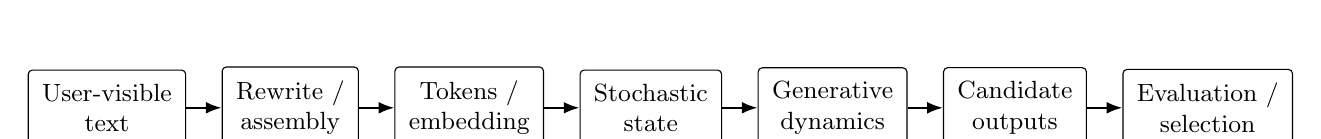
\begin{tikzpicture}[
node distance=0.45cm,
box/.style={draw, rounded corners=1.5pt, inner sep=5pt, font=\small, align=center, minimum height=0.62cm},
arr/.style={-{Latex[length=2mm]}, thick}
]
\node[box] (u) {User-visible\\text};
\node[box, right=of u] (r) {Rewrite /\\assembly};
\node[box, right=of r] (e) {Tokens /\\embedding};
\node[box, right=of e] (s) {Stochastic\\state};
\node[box, right=of s] (g) {Generative\\dynamics};
\node[box, right=of g] (o) {Candidate\\outputs};
\node[box, right=of o] (v) {Evaluation /\\selection};
\draw[arr] (u)--(r);
\draw[arr] (r)--(e);
\draw[arr] (e)--(s);
\draw[arr] (s)--(g);
\draw[arr] (g)--(o);
\draw[arr] (o)--(v);
\end{tikzpicture}
\caption{Possible loci of control in a prompted generative system. A surface prompt-output pair observes only the endpoints.}
\label{fig:layers}
\end{figure}

The causal question can be stated more precisely. Let \(P\) be the visible prompt and \(Y\) the selected output. Between them may be transformations \(R\), a model-relative representation \(E\), stochastic state \(Z\), generation dynamics \(G\), a candidate set \(C\), and a selection procedure \(S\):

\[
Y = S\big(C(G(E(R(P)), Z))\big).
\]

This is \emph{our} abstraction, not the formalism of any one cited system. Its purpose is diagnostic. If changing \(P\) changes \(Y\), that fact alone does not tell us whether the change operated through a semantic effect of the visible words, a different rewrite, a tokenizer boundary, an embedding displacement, a changed interaction with \(Z\), a trajectory difference during generation, or a different candidate being selected.

The problem becomes especially acute when the intermediate variables are inaccessible. Simonen et al.'s study of Midjourney ``default images'' is useful precisely because the authors are cautious about this point. They identify visually similar outputs produced from dissimilar prompts and show that recurrent default-like motifs occur in real use \citep{Simonen2026DefaultImages}. Yet Midjourney is proprietary. The observed recurrence can be real while its causal location remains unresolved. A training-data gap, hidden preprocessing, model representation, sampling process, or some interaction among them could produce superficially similar evidence. The phenomenon is more secure than its mechanism.

\section{Five fractures in the prompt-as-cause picture}

The field becomes more interesting when the disruptions are not collapsed into one story. They pull in different directions.

\subsection{The words you wrote may not be the words executed}

OpenAI's documented DALL-E 3 pipeline provides a clear architectural example: ChatGPT can expand an initial idea into a more detailed prompt before image generation \citep{OpenAI2023DALLE3}. In the API documentation for DALL-E 3, prompt rewriting was likewise described as a stage that optimizes prompts before they are passed downstream. Whatever one thinks of that design, it establishes a simple fact: a user-visible request and an executed image-model prompt can be different textual objects.

DSPy makes a related separation programmatic. Instead of treating a hand-written prompt template as the durable source artifact, DSPy represents language-model pipelines as text-transformation graphs containing declarative modules and compiles those programs to improve a specified metric \citep{Khattab2023DSPy}. The wording used at execution can therefore be an optimization product rather than the primary human-authored object.

These cases create a straightforward rival explanation for any prompt effect. Suppose two user prompts \(P_1\) and \(P_2\) produce different outputs. A surface-semantic account says the downstream model interpreted the difference between \(P_1\) and \(P_2\). A transformation account says an upstream mechanism mapped them to different effective instructions \(R(P_1)\) and \(R(P_2)\), and \emph{that} difference did the work. Conversely, two dissimilar user prompts can converge if \(R(P_1) \approx R(P_2)\). A downstream generator can then be perfectly responsive to its actual input while looking, from the interface, as though it ``defaulted.''

The distinction is not philosophical ornament. It changes the experiment required to support a claim about wording. If the transformed instruction is unobserved, a surface prompt comparison cannot distinguish interpretation by the generator from interpretation by the rewriter.

\subsection{Readable language is neither necessary nor sufficient for model-relative meaning}

A second fracture cuts deeper. Qin and Eisner show that language models can be queried using learned ``soft words'': continuous vectors that need not correspond to ordinary word embeddings \citep{QinEisner2021SoftPrompts}. Their prompts can be optimized by gradient descent, including from random initialization. Whatever human readability contributes to prompting, it is therefore not a necessary condition for effective model control.

The complementary anomaly appears on the human side. Milliere constructs nonce strings with no ordinary lexical standing that nonetheless evoke stable visual concepts in text-to-image models \citep{Milliere2022MadeUpWords}. Macaronic prompting exploits subword fragments across languages; evocative prompting exploits morphological resemblance. Struppek et al. show that replacing a single Latin character with a visually similar non-Latin character can systematically alter generated cultural attributes, and they locate the effect in the text encoder \citep{Struppek2023Homoglyphs}.

Taken together, these results break a tempting equivalence:

\[
\text{human meaningfulness} \neq \text{model-relative control strength}.
\]

A legitimate human word can be weakly represented. A human nonword can be operationally strong. A character whose substitution barely changes intended meaning can move the model in embedding space. A continuous vector can exert control without any readable word at all.

This does not mean that natural language is irrelevant. It means its special status must be stated more carefully. Natural language is a control surface that is simultaneously available to human interpretation and mapped into a model-relative representational geometry. Its practical force depends on the partial alignment of those two semantic systems. Prompt craft operates inside that alignment, but the alignment is neither complete nor stable across models.

\subsection{Representation can occur without surviving to the output}

A missing object in a final image is often treated as evidence that the model failed to ``understand'' the prompt. A-STAR complicates that inference. By inspecting cross-attention in text-to-image diffusion models, Agarwal et al. report that multiple requested concepts can overlap spatially such that one is ignored, and that concepts evident during early denoising can fail to be retained by later steps \citep{Agarwal2023ASTAR}. Their attention-segregation and attention-retention losses are interventions on these distinct failures.

The conceptual consequence is important even if cross-attention is not equated with human-like understanding. Final absence does not prove initial absence. A requested concept may have several different histories:

\begin{enumerate}[leftmargin=1.5em]
\item it never acquires a strong model representation;
\item it acquires representation but conflicts with another concept;
\item it becomes influential early and loses that influence later;
\item it remains represented but fails to determine visible output.
\end{enumerate}

These histories are observationally similar if one looks only at the final image. They imply different causal interventions. Better wording might help the first. Spatial attention control might help the second. Retention interventions might help the third. A final-output adherence score collapses all four.

This temporal problem matters for default-image research. A recurrent motif could be a pre-existing fallback reached when the requested concept never gains traction. Or it could be what remains after requested semantics initially participate and then lose a competition. The resulting image would be the same kind of evidence but the mechanism would be opposite: absence from the start versus extinction over time.

\subsection{Randomness is not necessarily semantically neutral after it enters a trained generator}

Prompt discussions often assign a clean division of labor: the prompt supplies semantics and the seed supplies variation. Simonen et al.'s seed ablations already make that division unstable. Fixed seeds make recurrent defaults easier to observe, while seed changes alter which motifs appear \citep{Simonen2026DefaultImages}. The real-world dataset, in which seeds vary, contains more motif variation than the fixed-seed manual experiment.

Mao et al. provide a mechanism showing why ``random variation'' may be too weak a description. In Stable Diffusion, they manipulate blocks of the initial latent noise and find that blocks exhibit preferences for generating particular content; moving those blocks can steer where content appears \citep{Mao2023InitialImageEditing}. The content is not intrinsic to Gaussian noise in isolation. It is a property of the relation between an initial state and a trained denoiser. But that is precisely the point. Once random state enters a learned dynamical system, semantically unequal futures can emerge from statistically sampled initial conditions.

This produces another rival causal story. Under strong prompt guidance, the marginal influence of initial state may be constrained. Under weak guidance, latent-state affordances and model priors may gain relative power. What looks like ``underspecification'' may therefore be less like leaving a blank and more like transferring causal authority to other variables.

The discriminating question is not whether seed matters; it obviously does. It is whether the causal effect of seed systematically increases as effective semantic control decreases. That interaction is testable.

\subsection{More words can mean less control}

The strongest practical assumption in prompt engineering may be monotonicity: if a behavior matters, specify it more clearly. Yang et al. directly pressure that intuition. In their study of underspecified LLM prompts, models sometimes satisfy requirements that were not stated, but those behaviors are less robust across prompt or model changes. At the same time, adding more requirements does not reliably improve performance because instruction following is limited and constraints compete \citep{Yang2025PromptsDontSay}. Their solution explicitly optimizes which requirements to state.

This result should not be reduced to ``short prompts are better.'' It reveals that written specification and effective control are not the same variable. A requirement may be:
\begin{itemize}[leftmargin=1.5em]
\item stated in prose;
\item supplied by a model default;
\item demonstrated through examples;
\item guaranteed by a decoding or grammar constraint;
\item checked by an evaluator after generation;
\item or absent from the behavior entirely.
\end{itemize}

The more interesting engineering question is therefore not how to put every requirement into the prompt. It is how to allocate requirements among control channels without creating interference. This again destabilizes causal attribution to words. A behavior can occur because it was written, because it was defaulted, or because another mechanism enforced it. The same output does not identify which one happened.

\section{Four rival accounts of prompt effects}

The findings above can be organized into four rival accounts. They are not mutually exclusive as system architectures; they are rival explanations for a \emph{particular observed prompt effect}. The same system may instantiate different accounts on different runs or for different features.

\begin{table}[ht]
\small
\centering
\begin{tabularx}{\textwidth}{>{\bfseries}p{0.17\textwidth} X X}
\toprule
Account & Where the decisive difference is located & What would discriminate it \\
\midrule
Surface-semantic & Human-visible wording changes the model's effective semantic conditioning in the intended direction. & Paraphrase, deletion, and clause interventions change the target behavior while downstream transformations and state are held fixed. \\
Transformation & Rewrite, compilation, retrieval, or prompt assembly creates the effective difference before the model interprets the request. & Log or control the transformed instruction; surface differences disappear when transformed state is held constant. \\
Distributed-dynamical & Output emerges from interaction among conditioning, model priors, stochastic state, and time-varying generative dynamics. & Prompt effects depend strongly on seed, latent interventions, or temporal retention; no surface clause has a stable marginal effect in isolation. \\
Selection & The decisive difference occurs after candidate generation through evaluation, ranking, user choice, or optimization. & Candidate distributions stay similar while changing evaluator or selection rule changes the surviving artifact or descendant prompt. \\
\bottomrule
\end{tabularx}
\caption{Rival causal explanations for an observed prompt effect.}
\label{tab:rivals}
\end{table}

The value of this taxonomy is not the labels. It is that each account requires different evidence. A prompt-output screenshot cannot distinguish them. Even an A/B test on prompt wording may not distinguish them if the rewrite system, random state, or selection policy changes as a consequence of the wording.

The accounts also interact with prompt optimization. Pryzant et al.'s Automatic Prompt Optimization generates natural-language criticisms of failures, treats them as textual ``gradients,'' rewrites prompts in the opposite semantic direction, and uses beam search and selection to retain better candidates \citep{Pryzant2023APO}. Promptbreeder goes farther by evolving task prompts and also the mutation prompts that generate their descendants \citep{Fernando2023Promptbreeder}. In these systems, the final wording can be causally downstream of a metric. The prompt is not only a cause of model behavior; it is itself an effect of an optimization environment.

This reversibility matters. The sentence that appears to be the source instruction may also be the surviving artifact of prior selection. Prompt provenance is therefore not merely historical bookkeeping. It is evidence about causal direction.

\section{Default images as a case of underdetermined causality}

Default images are particularly useful because they force the problem into view. Simonen et al. define the phenomenon operationally through a mismatch of relations: visually similar outputs arise from lexically and semantically dissimilar prompts \citep{Simonen2026DefaultImages}. Their computational pipeline clusters images using CLIP embeddings and then removes clusters whose prompts are too lexically or semantically similar. The phenomenon is not ``the image looks bad.'' It is convergence in output space despite divergence in instruction space.

That pattern is consistent with several mechanisms:

\begin{description}[leftmargin=1.6em,style=nextline]
\item[Weak-representation account.] Different prompts fail to activate strong distinct concepts, so generation falls toward common learned visual regions.
\item[Rewrite-convergence account.] Different visible prompts are mapped to similar effective instructions before image generation.
\item[Sampling-basin account.] Weak conditioning makes seed- and latent-specific basins more influential, producing recurring motifs for subsets of random states.
\item[Temporal-replacement account.] Weak requested concepts initially participate but lose control as recurrent motifs dominate later denoising.
\item[Measurement account.] Some apparent cluster structure is amplified by the geometry of the visual embedding used to detect similarity.
\end{description}

The last account is not a claim that Simonen et al.'s clusters are artifacts. Their manual affinity grouping gives evidence independent of the large-scale embedding pipeline. But Chowdhury et al. show that contrastive embedding spaces can contain hubs: candidates anomalously close to many queries \citep{Chowdhury2024NNN}. Simonen et al. use image-image CLIP similarity rather than exactly the image-text retrieval setting studied by Chowdhury et al., so the mechanisms are not identical. The important point is epistemic: the detector itself has a geometry that must be separated from the generator's geometry.

Default images therefore make a strong methodological lesson available without requiring one favored mechanism. A recurrent behavioral phenomenon can be established before its causal location is known. Research improves when it preserves that difference.

\section{The intervention ladder}

If prompt research wants causal claims rather than surface correlations, it needs experiments designed to locate effects. The following intervention ladder is a research program rather than a universal protocol. Each rung asks whether an apparent prompt effect survives after a different source of variation is controlled.

\subsection{1. Intervene on visible wording}

Begin with the ordinary prompt experiment, but make it genuinely contrastive. Use minimal deletions, substitutions, reordering, and paraphrases. Measure each requested property separately rather than relying on one holistic quality score. ChainForge's comparison-oriented design is useful here because it treats prompt variants and model responses as a field rather than a transcript \citep{Arawjo2023ChainForge}.

A clause counts as evidence of surface control only if its intervention has a reproducible, target-specific effect. If deleting a clause does nothing, the behavior attributed to that clause may be supplied elsewhere.

\subsection{2. Hold transformation constant}

Where rewriting or compilation exists, record it. Compare:
\[
P_1 \rightarrow R(P_1), \qquad P_2 \rightarrow R(P_2).
\]
Then create counterfactual runs in which \(P_1\) and \(P_2\) are forced to share the same downstream representation or transformed prompt. If the output difference vanishes, the causal locus has moved upstream or into transformation.

This is straightforward in inspectable systems and impossible in some proprietary ones. The impossibility is itself a result: causal claims about user wording should then be bounded accordingly.

\subsection{3. Intervene on representation}

The soft-prompt, nonce-word, and homoglyph results imply that visible lexical categories are insufficient. For open models, compare human-word and nonword prompts after tokenization and embedding. Construct matched cases:
\begin{enumerate}[leftmargin=1.5em]
\item human word, strong model association;
\item human word, weak model association;
\item human nonword, strong model association;
\item human nonword, weak model association;
\item continuous soft control with comparable downstream effect.
\end{enumerate}
If model behavior tracks representation strength better than lexical status, ``known word'' should be abandoned as a causal variable.

\subsection{4. Intervene through time}

For generative processes with inspectable intermediate states, record concept influence across the trajectory. The relevant question is not simply whether a token has high attention. It is whether targeted interventions at different timesteps change the probability that the concept survives to the output.

This distinguishes failure to acquire from failure to retain. A prompt can be effective early and ineffective late. ``The prompt worked'' then becomes temporally indexed.

\subsection{5. Intervene on stochastic state}

Cross prompt strength with fixed seed sets. Estimate prompt-by-seed interaction rather than treating seed as nuisance variance. In diffusion models, initial-latent interventions such as those demonstrated by Mao et al. offer stronger evidence than seed comparison alone \citep{Mao2023InitialImageEditing}. If the marginal effect of stochastic state increases as semantic guidance weakens, underspecification is literally a transfer of control.

\subsection{6. Intervene on evaluation and selection}

Finally, preserve the candidate set. Change only the evaluator, ranking metric, or human selection rule. Automatic prompt optimization and evolutionary prompting make this stage especially consequential \citep{Pryzant2023APO,Fernando2023Promptbreeder}. If candidate distributions remain similar while changing the evaluator produces different surviving artifacts or descendant prompts, authorship and control have moved downstream.

The intervention ladder produces a different kind of prompt receipt. Instead of recording only the successful sentence, it records which variables were held constant and which intervention produced the effect. That is not a new ontology of the prompt. It is a higher evidentiary standard for claims about what the prompt did.

\section{Three tensions that should remain unresolved}

A strong theory here should resist closing several questions that the evidence has only made sharper.

\subsection{Explicitness versus control}

Yang et al. make it difficult to preserve the intuition that better specification is simply more explicit specification \citep{Yang2025PromptsDontSay}. But the opposite slogan---``leave things implicit''---would be equally weak. Omitted requirements are less stable. The unresolved question is allocation: which properties should be expressed in prose, supplied by examples, encoded as formal constraints, delegated to model defaults, or enforced by tests?

This is a deeper problem than prompt length. It suggests that prompt practice sits inside a multi-channel control system. The relevant design variable may be not \emph{how much is written} but \emph{where each requirement is made operative}.

\subsection{Human language versus operative language}

Soft prompts, nonce strings, and homoglyphs jointly imply that a model's operative control geometry does not respect the borders of human vocabulary \citep{QinEisner2021SoftPrompts,Milliere2022MadeUpWords,Struppek2023Homoglyphs}. Yet human-readable prompting remains powerful and culturally consequential. Calling the underlying space a ``hidden language'' would be premature; tokenization and embedding geometry provide less mystical mechanisms for at least some effects.

The unresolved question is what relation should replace the idea of shared vocabulary. A promising formulation is alignment between two systems of difference: distinctions meaningful to people and distinctions that change model behavior. Prompt practice becomes interesting precisely where those systems line up imperfectly.

\subsection{Randomness versus semantics}

Mao et al. do not show that Gaussian noise contains concepts. They show that particular latent values, in relation to a trained generator, have content preferences \citep{Mao2023InitialImageEditing}. Simonen et al. do not show that seed is a semantic variable. They show that seed materially changes which recurrent defaults appear \citep{Simonen2026DefaultImages}. The unresolved question is whether ``semantic control'' should be reserved for language-mediated influence or generalized to any variable that systematically determines content.

The terminology matters because the causal fact may be easier than the conceptual one. It may be empirically demonstrable that seed assumes greater control under weak conditioning while remaining unclear whether that control deserves to be called semantic. A useful theory should permit the mechanism to be measured before the vocabulary is settled.

\section{What this changes about prompt practice}

The causal-attribution problem has practical consequences without requiring the stronger claim that visible language is unimportant.

First, prompt debugging should localize failure before prescribing better wording. If an upstream rewriter neutralized a distinction, editing the downstream description is misdirected. If a concept is represented and then lost, adding synonyms may not address the actual mechanism. If seed interactions dominate under weak control, judging a prompt from one sample conflates instruction with state.

Second, reproducibility should preserve the conditions under which a prompt effect was observed. Model version, transformation stage, stochastic state, candidate set, and selection procedure are not always available, but their absence should be represented as missing evidence rather than silently assigned to ``the prompt.''

Third, authorship questions become experimentally sharper. Promptbreeder and automatic prompt optimization reveal that wording can be generated by a search process whose metric determines survival \citep{Fernando2023Promptbreeder,Pryzant2023APO}. If changing the fitness function changes final behavior more than changing the initial wording, then attribution to the person who wrote the ancestor prompt is incomplete. Conversely, if final behavior remains highly sensitive to tiny human textual interventions after optimization and selection are held constant, linguistic authorship remains a powerful causal locus.

Fourth, creative prompt practice may resist classical experimentation because its objective can change when an output appears. ChainForge identifies modes of opportunistic exploration and iterative refinement alongside limited evaluation \citep{Arawjo2023ChainForge}. In creative work, a surprising artifact can alter what the practitioner wants. The output becomes a cause of the next criterion. A prompt history that preserves only text changes but not changes in the evaluator confuses a coupled discovery process with optimization toward a fixed target.

This is perhaps the most consequential reversal. Prompting does not only describe a desired world and cause a model to move toward it. Generated worlds can teach the prompter what was worth desiring. Causality loops back.

\section{Limits}

The sources assembled here concern different model families, interfaces, and research questions. They must not be merged into one mechanism. A-STAR's cross-attention findings in diffusion models do not explain Midjourney's proprietary behavior. DALL-E 3's documented prompt rewriting does not imply that every image system rewrites prompts. Soft prompting in language models does not prove that natural-language prompting is epiphenomenal. Mao et al.'s latent manipulation does not make initial noise intrinsically semantic. Hubness in contrastive retrieval does not invalidate CLIP-based image clustering. Yang et al.'s findings about software requirements do not imply that creative prompts should minimize explicit instruction.

The paper's claim is therefore methodological and conditional. These independent results establish enough distinct causal pathways that surface prompt-output association is often underdetermined. Which pathway matters in a given system must be shown, not assumed.

A second limitation is accessibility. The strongest causal tests require intermediate states that proprietary systems do not expose. Black-box prompt research can still establish behavioral regularities, as the default-image work demonstrates. It should simply distinguish behavioral claims from causal localization.

Finally, causality itself can be scale-dependent. A visible prompt may be indispensable at the interaction level even if its exact lexical details are not the dominant cause of a particular feature. Human-level authorship and component-level causal influence are different questions. The intervention ladder is meant to prevent one from being smuggled into the other.

\section{Conclusion: the question after the paper}

The attractive question of the last few years has been whether prompts are programs. The evidence here makes that question feel oddly early. It assumes that the prompt is a stable object whose relation to execution is already known.

A harder question comes first.

\begin{quote}
\emph{Under what conditions are the words visible to the user actually the cause of what the generative system does?}
\end{quote}

The current evidence does not supply one answer. It supplies rival mechanisms. Words may directly change effective semantic conditioning. They may be rewritten before execution. Their operational force may depend on token and embedding geometry that diverges from human lexical meaning. Their influence may decay during generation. Their effect may be amplified or overwhelmed by stochastic initial state. Explicit requirements may interfere with one another. The final artifact may be decided downstream by evaluators and selection.

That plurality is not a reason to abandon prompt research. It specifies the next version of it. Prompt effects should be treated as causal hypotheses about a layered, partially observed system. The experiment is no longer only ``change the words and see what happens.'' It is ``change the words, hold the other possible causes still, and find where the difference survives.''

The deepest possibility is that no stage wins. If control is genuinely interactional, then asking where the prompt's causal power resides may eventually prove as misleading as asking which single component of a dynamical system caused its trajectory. But that conclusion has not been earned yet. The field is more interesting before that closure. We first need experiments capable of telling us when the words matter, when they stop mattering, and what takes over when they do.

\section*{References}

\begin{thebibliography}{99}

\bibitem[Agarwal et al.(2023)]{Agarwal2023ASTAR}
Agarwal, A., Karanam, S., Joseph, K. J., Saxena, A., Goswami, K., and Srinivasan, B. V. (2023).
A-STAR: Test-time Attention Segregation and Retention for Text-to-image Synthesis.
\emph{Proceedings of the IEEE/CVF International Conference on Computer Vision}, 2283--2293.
\url{https://arxiv.org/abs/2306.14544}

\bibitem[Arawjo et al.(2023)]{Arawjo2023ChainForge}
Arawjo, I., Swoopes, C., Vaithilingam, P., Wattenberg, M., and Glassman, E. L. (2023).
ChainForge: A Visual Toolkit for Prompt Engineering and LLM Hypothesis Testing.
\url{https://arxiv.org/abs/2309.09128}

\bibitem[Beurer-Kellner et al.(2023)]{BeurerKellner2023LMQL}
Beurer-Kellner, L., Fischer, M., and Vechev, M. (2023).
Prompting Is Programming: A Query Language for Large Language Models.
\emph{PLDI 2023}. DOI: 10.1145/3591300.

\bibitem[Chowdhury et al.(2024)]{Chowdhury2024NNN}
Chowdhury, N., Wang, F., Shenoy, S., Kiela, D., Schwettmann, S., and Thrush, T. (2024).
Nearest Neighbor Normalization Improves Multimodal Retrieval.
\url{https://arxiv.org/abs/2410.24114}

\bibitem[Fernando et al.(2023)]{Fernando2023Promptbreeder}
Fernando, C., Banarse, D., Michalewski, H., Osindero, S., and Rocktaschel, T. (2023).
Promptbreeder: Self-Referential Self-Improvement Via Prompt Evolution.
\url{https://arxiv.org/abs/2309.16797}

\bibitem[Khattab et al.(2023)]{Khattab2023DSPy}
Khattab, O., Singhvi, A., Maheshwari, P., Zhang, Z., Santhanam, K., Vardhamanan, S., Haq, S., Sharma, A., Joshi, T. T., Moazam, H., Miller, H., Zaharia, M., and Potts, C. (2023).
DSPy: Compiling Declarative Language Model Calls into Self-Improving Pipelines.
\url{https://arxiv.org/abs/2310.03714}

\bibitem[Liang et al.(2025)]{Liang2025PromptsPrograms}
Liang, J. T., Lin, M., Rao, N., and Myers, B. A. (2025).
Prompts Are Programs Too! Understanding How Developers Build Software Containing Prompts.
\emph{Proceedings of the ACM on Software Engineering}, 2.
DOI: 10.1145/3729342.

\bibitem[Mao et al.(2023)]{Mao2023InitialImageEditing}
Mao, J., Wang, X., and Aizawa, K. (2023).
Guided Image Synthesis via Initial Image Editing in Diffusion Model.
\url{https://arxiv.org/abs/2305.03382}

\bibitem[Milliere(2022)]{Milliere2022MadeUpWords}
Milliere, R. (2022).
Adversarial Attacks on Image Generation With Made-Up Words.
\url{https://arxiv.org/abs/2208.04135}

\bibitem[OpenAI(2023)]{OpenAI2023DALLE3}
OpenAI. (2023).
DALL-E 3.
\url{https://openai.com/index/dall-e-3/}

\bibitem[Pryzant et al.(2023)]{Pryzant2023APO}
Pryzant, R., Iter, D., Li, J., Lee, Y. T., Zhu, C., and Zeng, M. (2023).
Automatic Prompt Optimization with ``Gradient Descent'' and Beam Search.
\url{https://arxiv.org/abs/2305.03495}

\bibitem[Qin and Eisner(2021)]{QinEisner2021SoftPrompts}
Qin, G. and Eisner, J. (2021).
Learning How to Ask: Querying LMs with Mixtures of Soft Prompts.
\url{https://arxiv.org/abs/2104.06599}

\bibitem[Simonen et al.(2026)]{Simonen2026DefaultImages}
Simonen, H., Kiviniemi, A., Johnston, H., Barranha, H., and Oppenlaender, J. (2026).
An Exploration of Default Images in Text-to-Image Generation.
\emph{Proceedings of the 2026 CHI Conference on Human Factors in Computing Systems}.
DOI: 10.1145/3772318.3790681.

\bibitem[Struppek et al.(2023)]{Struppek2023Homoglyphs}
Struppek, L., Hintersdorf, D., Friedrich, F., Brack, M., Schramowski, P., and Kersting, K. (2023).
Exploiting Cultural Biases via Homoglyphs in Text-to-Image Synthesis.
\emph{Journal of Artificial Intelligence Research}, 78, 1017--1068.
\url{https://arxiv.org/abs/2209.08891}

\bibitem[Yang et al.(2025)]{Yang2025PromptsDontSay}
Yang, C., Shi, Y., Ma, Q., Liu, M. X., Kastner, C., and Wu, T. (2025).
What Prompts Don't Say: Understanding and Managing Underspecification in LLM Prompts.
\url{https://arxiv.org/abs/2505.13360}

\end{thebibliography}

\appendix
\section{Assembly and provenance}

This manuscript was assembled from a preserved research corpus of 21 immutable zettel payloads and a local copy of Simonen et al.'s CHI 2026 paper. During this revision, primary source pages for key technical claims were independently checked where accessible. The prior paper, \emph{The Prompt Is Not the Program: Execution Lineage and the New Unit of Prompt Practice}, was retained as a prior derived interpretation but was not used as the organizing thesis.

The current assembly instrument is:
\begin{verbatim}
_PROMPTS/ANCIENT_MASTER_SLIPCASE_v15.6-TENSION-FIRST__assembly-prompt.txt
\end{verbatim}

The package also contains:
\begin{verbatim}
000__TENSIONS.txt
000__DEEP_QUESTIONS.txt
000__PAPER_STATE.txt
when-words-stop-being-the-cause__SOURCE_MAP.txt
000__RETURN_PATH.txt
000__MAKING_HISTORY.txt
\end{verbatim}

The paper is a current wager, not an evidentiary source. Its central question remains open.

\end{document}
